\documentclass{article}
\usepackage{graphicx}
\usepackage{booktabs}
\usepackage{hyperref}
\usepackage{geometry}
\geometry{margin=1in}

\title{Enhancing Output Uniqueness in Large Language Models via Model Rotation, Temperature Tuning, and Embedding-Based Validation}
\author{Sushanth Tiruvaipati \\ \small Kreative Koala LLC}
\date{}

\begin{document}

\maketitle

\begin{abstract}
We present a lightweight, practical method to increase the uniqueness of outputs generated by large language models (LLMs). Our approach combines: (1) temperature sampling, (2) rotation between diverse LLM APIs, (3) embedding-based uniqueness validation, and (4) an in-production deduplication pipeline. We compare six production-grade LLMs (GPT-4, GPT-4-Turbo, GPT-3.5-Turbo, Claude-3-Sonnet, Gemini-Pro, and DeepSeek), analyze cost-vs-uniqueness trade-offs, and propose a metric for uniqueness using cosine similarity between embedding vectors of generated outputs. We show that controlled rotation combined with moderate temperature tuning can significantly enhance output variability while staying within acceptable cost and quality bounds.
\end{abstract}

\section{Introduction}
Modern LLMs like GPT-4 and Claude-3 produce high-quality responses, but often converge on similar outputs when presented with identical prompts. This behavior is useful for reliability but problematic when diversity or creativity is desired. In applications such as content generation, puzzle creation, or brainstorming, uniqueness becomes a key quality signal.

We explore simple yet effective strategies to amplify uniqueness:
\begin{itemize}
  \item Temperature variation
  \item Model rotation (cycling across multiple providers)
  \item Embedding-based uniqueness validation
  \item Production-grade duplicate detection logic
\end{itemize}

\section{System Architecture}
Our Node.js service supports multiple LLMs, rotating across APIs, collecting responses, validating uniqueness using MiniLM embeddings, and tracking cost. Duplicate detection uses structural JSON checks and embedding similarity scoring.

\section{Methodology}
\begin{itemize}
  \item \textbf{Temperature Sweeps:} Range from 0.1 to 1.3
  \item \textbf{Model Rotation:} Round-robin sampling across LLMs
  \item \textbf{Uniqueness Metric:} Cosine distance of sentence embeddings
  \item \textbf{Cost Tracking:} Price-normalized token accounting
\end{itemize}

\section{Results}
\subsection*{Temperature vs Creativity (GPT-4)}
\begin{center}
\begin{tabular}{lcccccc}
\toprule
Temperature & Uniqueness & Validation & Duplicates & Cost (\$) & Efficiency \\
\midrule
0.1 & 0.1293 & 1.0000 & 1.0000 & 0.0253 & 39.46 \\
0.3 & 0.1787 & 1.0000 & 1.0000 & 0.0242 & 41.40 \\
0.5 & 0.1961 & 1.0000 & 0.8000 & 0.0259 & 38.67 \\
0.7 & 0.2425 & 1.0000 & 0.6000 & 0.0257 & 38.90 \\
0.9 & 0.2494 & 1.0000 & 0.3333 & 0.0270 & 37.06 \\
1.1 & 0.2753 & 1.0000 & 0.4000 & 0.0286 & 34.92 \\
1.3 & 0.4220 & 0.9767 & 0.0667 & 0.0398 & 24.54 \\
\bottomrule
\end{tabular}
\end{center}

\begin{figure}[h!]
  \centering
  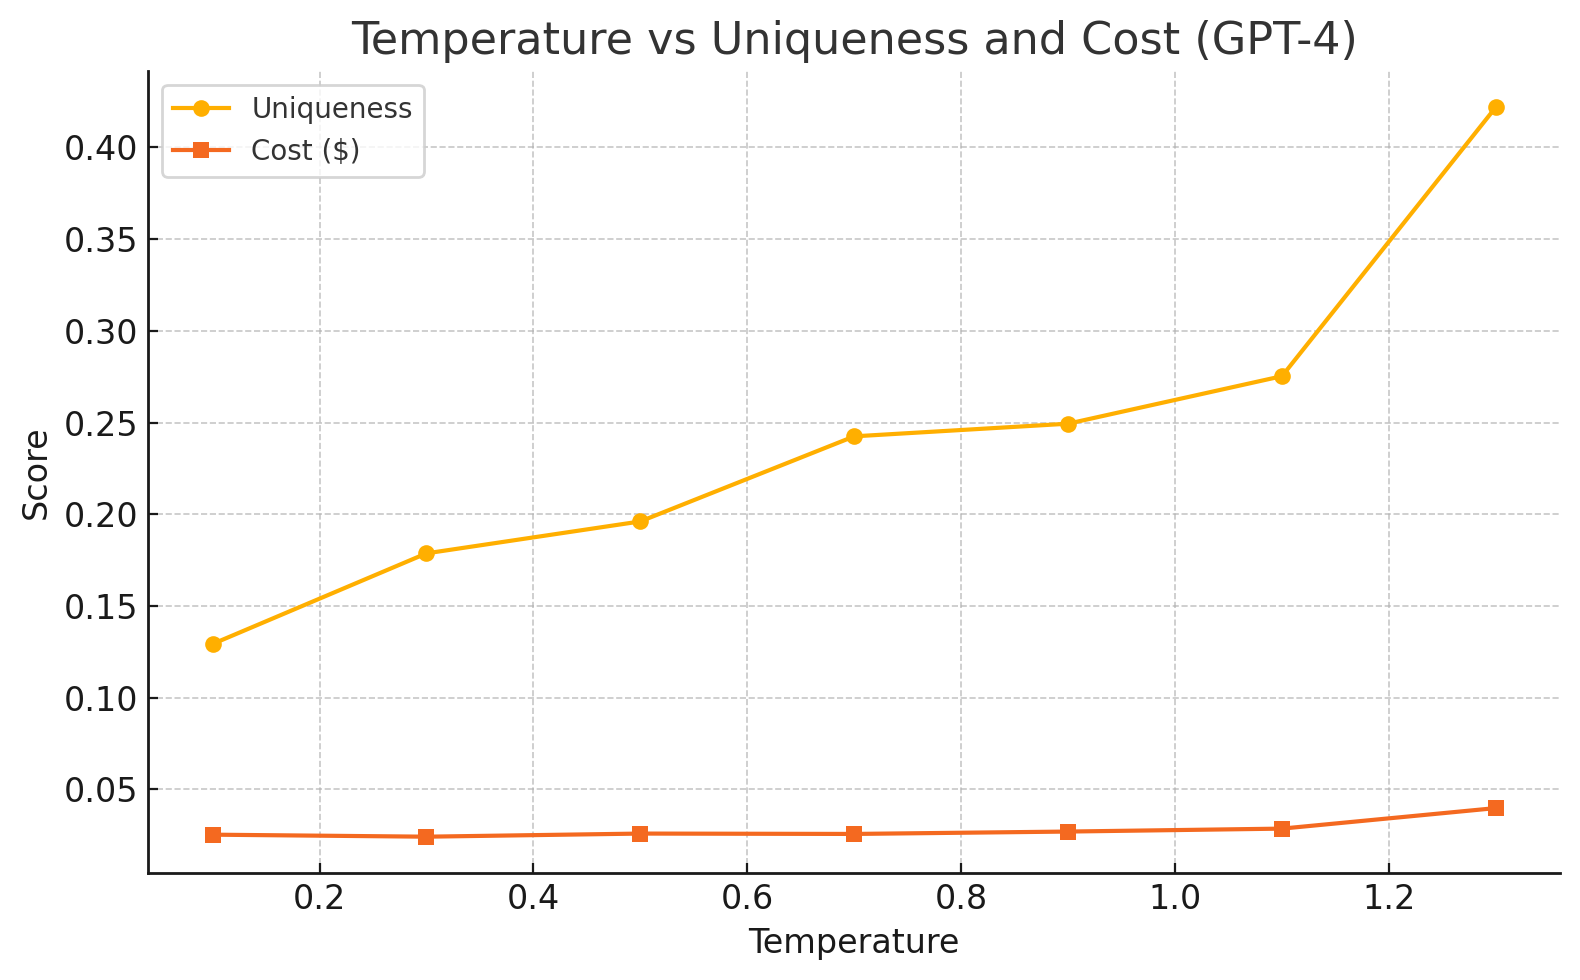
\includegraphics[width=0.75\linewidth]{temperature_plot.png}
  \caption{Temperature vs Uniqueness and Cost (GPT-4)}
  \label{fig:temperature_plot}
\end{figure}

\section{Discussion}
Model rotation improves diversity beyond temperature tuning alone. Embedding-based scoring proves useful for rapid validation. The best trade-off between creativity and cost appears at temperatures between 0.7–0.9. Our system is efficient and extensible for production use.

\section{Conclusion}
We enhance LLM output uniqueness using simple strategies such as temperature tuning and model rotation. These methods yield measurable improvements in uniqueness while keeping cost and quality within acceptable limits. Our framework, metrics, and results are open-sourced for further experimentation.

\section*{References}
\begin{itemize}
  \item OpenAI Pricing: \url{https://openai.com/pricing}
  \item Sentence Transformers: \url{https://www.sbert.net}
  \item Anthropic Claude API: \url{https://docs.anthropic.com}
  \item Gemini API: \url{https://ai.google.dev}
  \item DeepSeek API: \url{https://deepseek.com}
\end{itemize}

\end{document}

